\ifdefined\THESIS
    \chapter{\uppercase{Evaluation}}
\else
    \section{Evaluation}
\fi

We evaluate the system against several baseline implementations, and evaluate
how the performance of the system varies with the number of contacts a user has
and how many FriendlyLocation chooses to use.
We used five-fold cross validation on the geo-located users to evaluate the system.
We evaluated the FriendlyLocation system against FIXME users.
FIXME users from this set were removed because none of their friends or
followers had decodable locations.


\begin{figure}[tb]
\centering
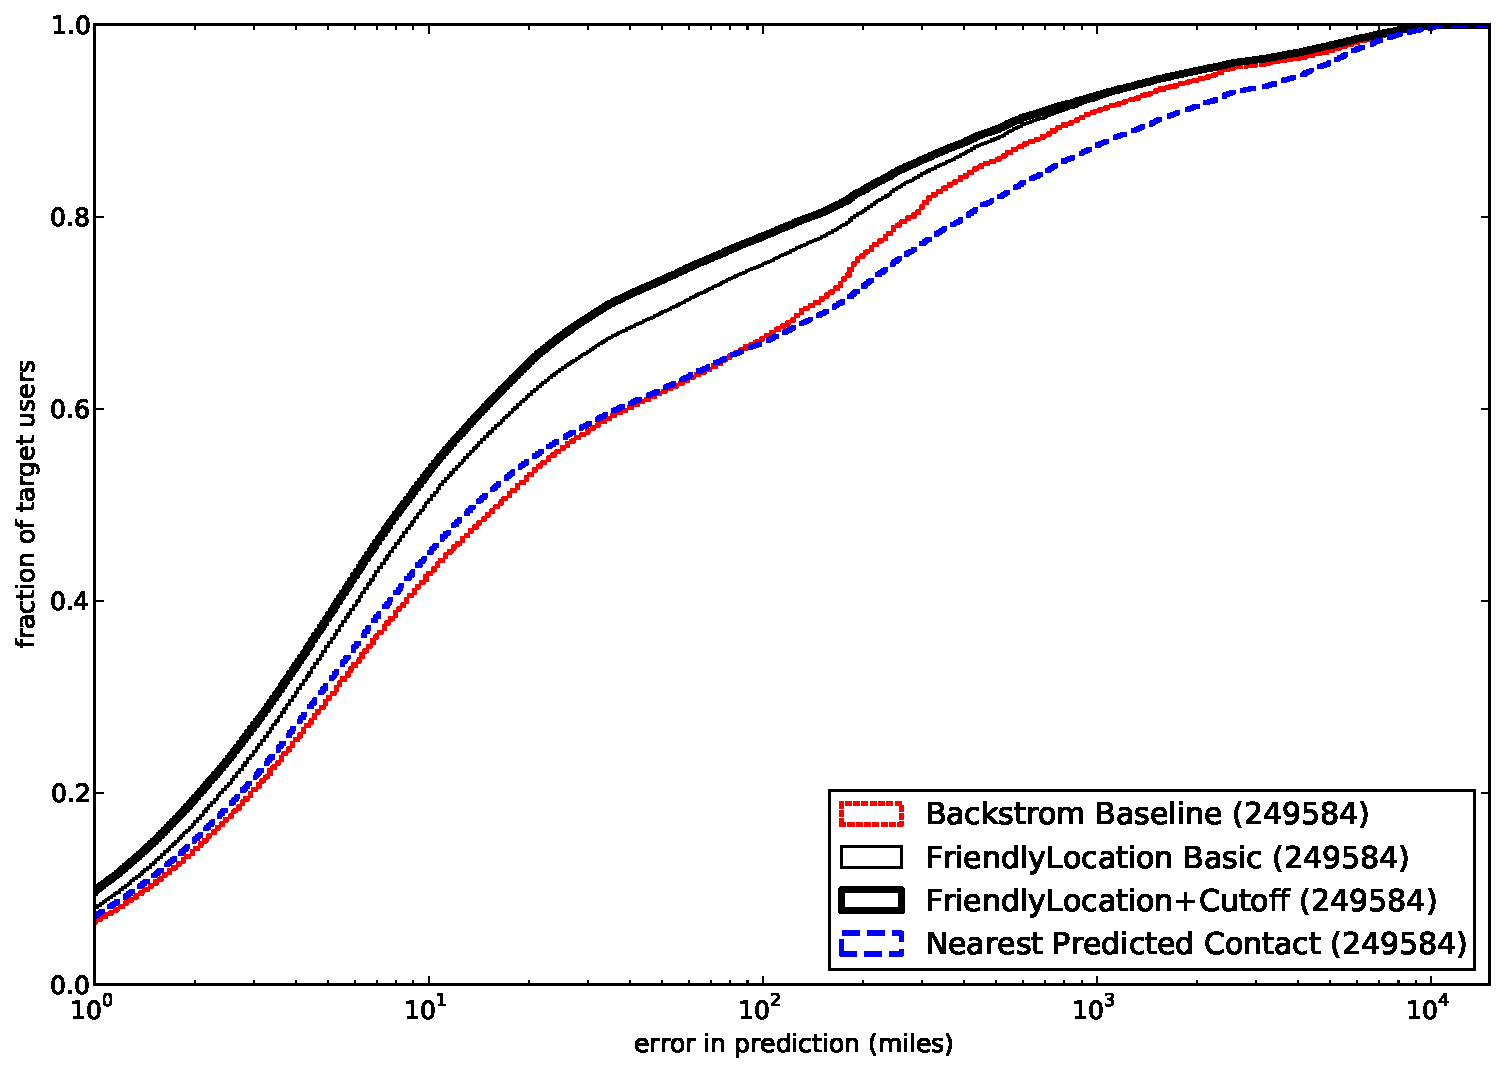
\includegraphics[width=\linewidth]{figures/fl_basic.pdf}
\caption{
    FriendlyLocation against several baseline systems.
    FIXME: remove some of these lines
}
\label{fig:NearProbFit}
\end{figure}

\begin{table}[tb]
\centering
\begin{tabular}{l  r r r r}
    Model
    & aed@60
    & aed@80
    & aed@100
    & acc@25 \\
    \hline
    Baseline & 8.41$\pm$.039 & 40.8$\pm$.20 & 426$\pm$3.8 & 55.7\%$\pm$.09\% \\
    FriendLoc & 5.43$\pm$.030 & 21.4$\pm$.15 & 359$\pm$3.8 & 63.9\%$\pm$.11\% \\
    Nearest & 7.50$\pm$.072 & 47.8$\pm$.52 & 573$\pm$4.5 & 56.9\%$\pm$.17\% \\
\end{tabular}
\caption{
results with standard deviation from five-fold cross validation
FIXME: explain this
}
\label{tab:results}
\end{table}

\subsection{Prediction}
We investigate several implementations of the FriendlyLocation system:
\begin{description}
%\item[FriendlyLocation Full] The MLE presented in the previous section with
%    additional information sources: UTC offset, the user-supplied location,
%    and the location of users who are not contacts.
\item[FriendlyLocation] This is the system described in the previous
    section with only information from the locations of contacts.
%\item[Median] Finds the median of the latitude and the median of the longitude
%f the 25 randomly selected contacts.
\item[Backstrom] This is based on the MLE estimator presented in
    \cite{backstrom2010find}. Some changes to the system were made to make it
    work. (FIXME: more here)
\item[Omniscient] Returns the location of the contact that is closest to the
    geo-located user from the 25 users used for location prediction.
\item[Random] Returns the location of a randomly-selected contact.
\end{description}

Our basic FriendlyLocation system predicts the location within 25 miles FIXME\% of
the time.
%
Our basic system preforms significantly better than the baseline implementations.
%
Unfortunately, when the predictor is wrong, it can be very wrong.
%
The comparison to the omniscient predictor shows that there is room for improvement.
%
Many users who have an incorrectly predicted location have at least one contact
that is closer than the incorrectly predicted location.


\section{Additional Information}
We investigated the effect of increasing numbers of contacts on the quality of
the results.

Before removing contacts without location information, we sorted the users into
groups based on the number of contacts the had.
Next, we ran the FriendlyLocation predictor against each of them.
Figure~\ref{fig:LulResults} shows the results of prediction.
The quality of the results from the predictor was lower for users with fewer
than 50 contacts; however, as contacts increased beyond that, it had no
significant effect on the results.

\ifdefined\THESIS
    Many Twitter users fill out the text-based location field.
    %
    If this user-reported data is good, there is no reason to spend time
    crawling their contacts.
    %
    It would be nice to use this information when predicting location, but
    the geo-located users we used to do the evaluation are less concerned about
    the privacy of their location information than the average Twitter user.
    %
    As a result, they tended to give more precise information in the location
    field of their user profile than other users.
    %
    We assume that the locations supplied by the contacts are more
    representative of normal Twitter users so we added noise to the locations
    of the geo-located users to make the distribution of the quality of their
    locations would match the quality of the contacts.
    %
    First, we sorted all the geo-located users and all the contacts by their
    PLE(predicted location error).
    %
    Next, we looked at each percentile of the geo-located users and compared
    their PLE to the PLE for that percentile in the contacts.
    %
    For each of the geo-located users, we moved the user's location based on
    reverse geocoding away from the user's actual median location based on the
    difference between the PLEs.
    %
    For example, the median PLE for a geo-located user was FIXME, and the median
    PLE for a contact was FIXME miles.
    %
    This means that we need to add FIXME miles of noise to a geo-located user
    with a PLE of FIXME.
    %
    We also removed the location field from FIXME\% of the geo-located users to
    make the proportion of geo-located users with a location match the general
    Twitter population.
\fi

FIXME: discuss adding other factors
FIXME: do we want to do us-only evaluation?

The final step of the evaluation is to investigate if FriendlyLocation would
work with a smaller number of profiles than 25.
%
FIXME: eval for small number of hand-picked and random contacts
%
In general, using more contacts can produce better results.
%
Although we limited the crawler to 25 randomly-picked contacts per geo-located
user, if FriendlyLocation is going to be used as part of a larger system, the
crawler should pick users based on relationship type before crawling.



